\documentclass[12pt]{article}

% Paquetes
\usepackage[spanish]{babel} 
\usepackage{graphicx}        

% Información del documento
\title{\textbf{\textit{TRABAJO PRÁCTICO PROTOCOLO IPv6}}}
\author{\textbf{Valentino Aviani y Luca Mamani} \\ \textbf{5to Informática}}

\begin{document}
	
	\maketitle 
	
	\begin{abstract}
		\textbf{Enlace al repositorio:} https://github.com/valentinoaviani14/redes.git 
		
		\textbf{Carpeta de imágenes:} tpipv6-2/imagenes
		
		\textbf{Carpeta del código:} proyectoLatex/TP2IPv6.tex
	\end{abstract}
	
	\tableofcontents
	
	\newpage  % Salto de página
	
	\begin{center}
		\section{CONFIGURACIÓN DE IPv6 SOBRE IPv4 UTILIZANDO GRE TUNNELS}
	\end{center}
	
	\subsection{INTRODUCCIÓN}
	{\large Los túneles GRE (Generic Routing Encapsulation) son un mecanismo que permite la transmisión de paquetes de diferentes protocolos a través de una red que solo soporta protocolos específicos. En términos de IPv4 e IPv6, GRE se usa para crear conexiones virtuales entre dos puntos de una red, ofreciendo una vía segura y eficiente para transmitir tráfico.}
	
	{\large En una red que utiliza IPv6 sobre un túnel GRE, el proceso de encapsulación permite que los paquetes IPv6 se transmitan por redes que aún operan con IPv4. Esto es especialmente útil durante la transición hacia IPv6, ya que permite interconectar diferentes tipos de redes mientras se garantiza la interoperabilidad entre los dos protocolos.}
	
	{\large Este documento detalla los pasos necesarios para configurar un túnel IPv6 sobre una red IPv4, utilizando dispositivos Cisco en un entorno simulado como \textit{Cisco Packet Tracer}.}
	
	\section{TOPOLOGÍA DE RED}
	
	{\large La topología utilizada consiste en dos routers conectados a través de una red IPv4, cada uno con una PC en su LAN interna. El túnel GRE conecta ambos routers para permitir comunicación IPv6.}
	
	\begin{figure}[h!]
	\centering
	\includegraphics[width=0.7\textwidth]{../tpipv6-2/imagenes/topologia}
	\caption{Topología utilizada en Cisco Packet Tracer}
	\end{figure}
	
	\section{CONFIGURACIÓN DE INTERFACES IPv4}
	{\large Se asignan direcciones IPv4 a las interfaces físicas de los routers para establecer la conectividad básica, sobre la cual se montará el túnel.}
	
	{\large R0:}
	
	\begin{figure}[h!]
		\centering
		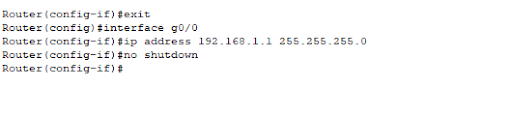
\includegraphics[width=0.7\textwidth]{../tpipv6-2/imagenes/confipv4r0}
		\caption{Cisco Packet Tracer}
	\end{figure}
	
	{\large R1:}
	
	\begin{figure}[h!]
		\centering
		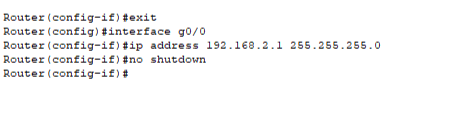
\includegraphics[width=0.7\textwidth]{../tpipv6-2/imagenes/confipv4r1}
		\caption{Cisco Packet Tracer}
	\end{figure}
	
	\newpage
	
	\section{HABILITAR EL ENRUTAMIENTO IPv6}
	{\large Es necesario habilitar el reenvío de paquetes IPv6.}
	
	\begin{figure}[h!]
		\centering
		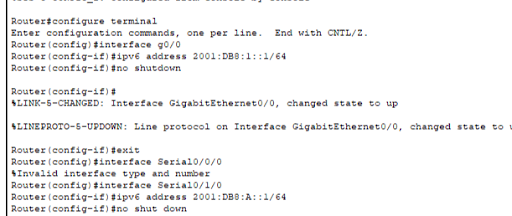
\includegraphics[width=0.7\textwidth]{../tpipv6-2/imagenes/confipv6r0}
		\caption{Cisco Packet Tracer}
	\end{figure}
	
	\begin{figure}[h!]
		\centering
		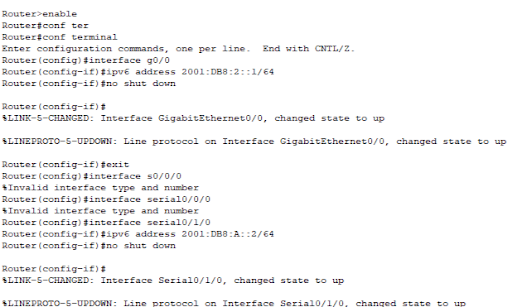
\includegraphics[width=0.7\textwidth]{../tpipv6-2/imagenes/confipv6r1}
		\caption{Cisco Packet Tracer}
	\end{figure}
	
	\section{DESACTIVACIÓN DE STP}
	{\large En algunos entornos de simulación como \textit{Cisco Packet Tracer}, la existencia del protocolo STP puede provocar bloqueos temporales o comportamiento inesperados, si hay enlaces redundantes entre switches.}
	
	\begin{figure}[h!]
		\centering
		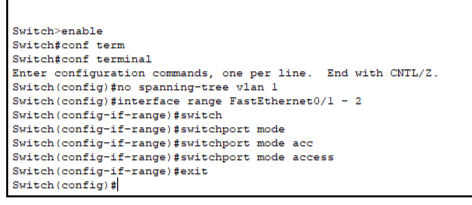
\includegraphics[width=0.7\textwidth]{../tpipv6-2/imagenes/stpsw1}
		\caption{Cisco Packet Tracer}
	\end{figure}
	
	\begin{figure}[h!]
		\centering
		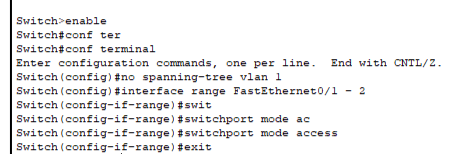
\includegraphics[width=0.7\textwidth]{../tpipv6-2/imagenes/stpsw0}
		\caption{Cisco Packet Tracer}
	\end{figure}
	
	\newpage
	
	\section{CONFIGURACIÓN DE LAS PCs}
	{large Cada PC de la red debe configurarse con una dirección IPv6 estática y su puerta de enlace por defecto para que puedan comunicarse a través del túnel GRE.}
	
	\begin{figure}[h!]
		\centering
		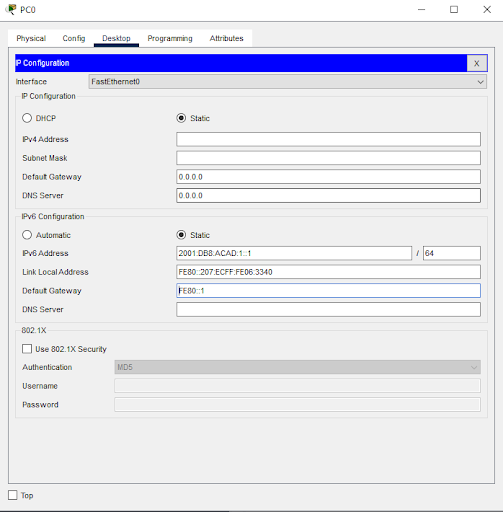
\includegraphics[width=0.7\textwidth]{../tpipv6-2/imagenes/confipv6pc0}
		\caption{Cisco Packet Tracer}
	\end{figure}
	
	\newpage
	
	\section{CREAR LA INTERFAZ DE TÚNEL}
	{\large Creamos una interfaz de túnel en cada router y le asignamos una dirección IPv6.}
	
	\begin{figure}[h!]
		\centering
		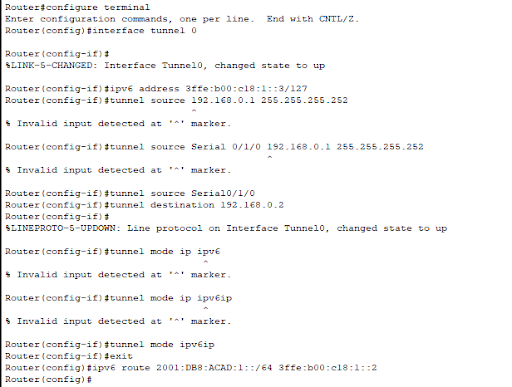
\includegraphics[width=0.7\textwidth]{../tpipv6-2/imagenes/conftunnelr0}
		\caption{Cisco Packet Tracer}
	\end{figure}
	
	\begin{figure}[h!]
		\centering
		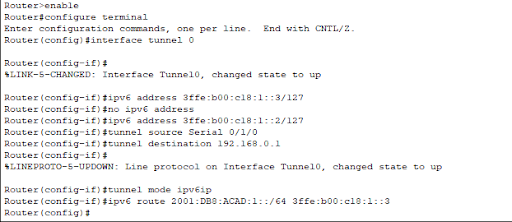
\includegraphics[width=0.7\textwidth]{../tpipv6-2/imagenes/conftunnelr1}
		\caption{Cisco Packet Tracer}
	\end{figure}
	
	\newpage
	
	\section{VERIFICACIÓN DE CONECTIVIDAD IPv6}
	{\large Ahora, veamos qué pasa si hacemos un ping a PC1 desde PC0:
	}
	
	{\large 1 -  En primera instancia, se puede observar que el paquete que sale de PC0 tiene de cabecera IPv6 de origen 2001:db8 :acad:1::1 y de destino la  IPv6 de la PC1: 2001:db8:acad:2::1. El tipo de mensaje es Echo request (128) y va dirigido al router0.}
	
	{\large 2 - Ahora, en router0, se puede observar que este le ingreso la información IPv4 al paquete para que pase por el túnel que se creo con Router1 en la red 192.168.0.0/30. El paquete tiene de ip de origen la ip del router0 y de destino la ip del router1. las ipv6 no cambian y el mensaje sigue siendo Echo Request (128).}
	
	{\large 3 - Luego de pasar por el túnel, router1 descarta la informacion de IP de origen y de destino del paquete y está preparado para pasar por la red IPv6 que tiene con PC1, pasando primero por el switch.
	}
	
	{\large 4 - Una vez recibido el mensaje, PC1 envía un nuevo mensaje de tipo Echo Reply (129), con IPv6 de destino a PC0. A partir de este punto se repite el proceso en todo recorrido de vuelta, con el único cambio de que el mensaje ahora es Echo Reply y no Request
	}
	
	{\large 5 - Finalmente,PC0 recibe exitosamente el mensaje Echo Reply de PC1 pasando correctamente por la conexión de túnel entre Router0 y Router1, por lo que podemos concluir en que todas las conexiones y configuraciones estan correctamente hechas.}
	
	
	\section {CONCLUSIÓN}
	{\large A lo largo de este trabajo se ha demostrado cómo implementar un túnel GRE para encapsular tráfico IPv6 sobre una infraestructura IPv4. Esta técnica resulta fundamental en escenarios donde estos protocolos deben coexistir.
		
		La configuración de los routers, la asignación de direcciones IPv6 en las PCs, y la correcta definición de las interfaces del túnel permiten una comunicación efectiva punto a punto mediante direcciones IPv6, incluso cuando el enlace físico intermedio utiliza exclusivamente IPv4.
		
		Además, trabajamos otros aspectos como la desactivación del protocolo STP en switches para evitar problemas de redundancia y bucles innecesarios en redes simulaciones.
		
		Este tipo de soluciones reflejan cómo pueden coexistir ambos protocolos y facilitan una transcición progresiva hacia IPv6.]
	
\end{document}
